\documentclass{beamer}
\usetheme{metropolis}
\usepackage{graphicx}
\usepackage{subfig}
\usepackage{tcolorbox}
\title{Algebra-Based Physics: Electricity, Magnetism, and Modern Physics (PHYS135B): Unit 0}
\author{Jordan Hanson}
\institute{Whittier College Department of Physics and Astronomy}

\begin{document}
\maketitle

\section{Summary}

\begin{frame}{Unit 0 Summary}
\textbf{Reading: Chapters 3.1 - 3.3, 18.1 - 18.5, 19.1 - 19.3}
\begin{enumerate}
\item Estimation/Approximation
\item Coordinates and Vectors
\item Review of concepts from Newtonian mechanics
\begin{itemize}
\item Kinematics and Newton's Laws
\item Work-energy theorem, energy conservation
\item Momentum, conservation of momentum
\end{itemize}
\item Electrostatics I: charges and fields
\item Electrostatics II: potential, and potential energy
\end{enumerate}
\end{frame}

\section{Estimation/Approximation}

\begin{frame}{Estimation/Approximation}
In science and engineering, \alert{estimation} is to obtain a quantity in the absence of precision, informed by rational constraints.
\begin{enumerate}
\item \textbf{Define relevant \alert{unit scales}}: (mg, g, or kg), (m/s or km/hr)
\item \textbf{Obtain \alert{complex quantities}} from simple ones
\begin{itemize}
\item Obtain \textit{areas} and \textit{volumes} from \textit{lengths}
\item Obtain \textit{rates} from \textit{numerators} and \textit{denominators}
\end{itemize}
\item \textbf{Taking advantage of \alert{scaling problems}}
\begin{itemize}
\item Knowing \textit{relationship} between variables
\item Using that \textit{relationship} to obtain new information
\end{itemize}
\item \textbf{Constrain the unknown with \alert{upper} and \alert{lower} limits}
\end{enumerate}
\end{frame}

\begin{frame}{Estimation/Approximation}
\textbf{Unit scale}: A generation is about one-third of a lifetime. Determine how many generations have passed since the year 0 AD\footnote{What is the appropriate scale here?}.
\begin{itemize}
\item A: $10$
\item B: $20$
\item C: $60$
\item D: $100$
\end{itemize}
\end{frame}

\begin{frame}{Estimation/Approximation}
\textbf{Unit scale}: (a) What fraction of Earth’s diameter\footnote{The diameter of the Earth is 12,800 km.} is the greatest ocean depth (11 km below sea level)? (b) The greatest mountain height (8.8 km above sea level)?
\begin{itemize}
\item A: $8.6 \times 10^{-2}$, $6.9 \times 10^{-2}$
\item B: $8.6 \times 10^{-3}$, $6.9 \times 10^{-3}$
\item C: $8.6 \times 10^{-4}$, $6.9 \times 10^{-4}$
\item D: $8.6 \times 10^{-5}$, $6.9 \times 10^{-3}$
\end{itemize}
\end{frame}

\begin{frame}{Estimation/Approximation}
\textbf{Complex quantities}: Assuming one nerve impulse must end before another can begin, what is the maximum firing rate of a nerve in impulses per second? 
\begin{itemize}
\item A: 1 per second (1 Hz)
\item B: 30 per second (30 Hz)
\item C: 60 per second (60 Hz)
\item D: 100 per second (100 Hz)
\end{itemize}
\end{frame}

\begin{frame}{Estimation/Approximation}
\textbf{Complex quantities}: If a Whittier College athlete ran the 5k race at a track meet in 35 minutes, what was her average speed?
\begin{itemize}
\item A: 0.3 meters per second
\item B: 3 meters per second
\item C: 30 meters per second
\item D: 300 meters per second
\end{itemize}
\end{frame}

\begin{frame}{Estimation/Approximation}
\textbf{Complex quantities}: Suppose you won the lottery and received \$1 billion USD.  Because your life is dope, you stack that paper over the Whittier College soccer field.  Each stack contains 100 bills, and each bill is worth \$100.  If you evenly cover the field, how high is the money level?
\begin{itemize}
\item A: 0.5 inch
\item B: 1 inch
\item C: 2 inches
\item D: 1 foot
\end{itemize}
\end{frame}

\begin{frame}{Estimation/Approximation}
\textbf{Scaling problem}: Supposed you have an ideal gas in a cylinder of fixed volume.  If the pressure begins as 100 kPa, and you \textit{double} the temperature of the gas, what is the new pressure?
\begin{itemize}
\item A: 100 kPa
\item B: 50 kPa
\item C: 10 kPa
\item D: 200 kPa
\end{itemize}
\end{frame}

\begin{frame}{Estimation/Approximation}
\textbf{Scaling problem}: Supposed you have an ideal gas in a cylinder of fixed volume.  If the pressure begins as 100 kPa, and you \textit{halve} the temperature of the gas, what is the new pressure?
\begin{itemize}
\item A: 100 kPa
\item B: 50 kPa
\item C: 10 kPa
\item D: 200 kPa
\end{itemize}
\end{frame}

\begin{frame}{Estimation/Approximation}
\textbf{Upper/lower limits}: How many undergraduate students are there at Whittier College\footnote{What is the absolute lower limit, and what is the upper limit?}?
\begin{itemize}
\item A: 5,000
\item B: 1,000
\item C: 1,250
\item D: 500
\end{itemize}
\end{frame}

\begin{frame}{Estimation/Approximation}
\textbf{Upper/lower limits}: What is the average yearly college tuition in the United States (before subtracting grants and scholarships)?
\begin{itemize}
\item A: \$5,000
\item B: \$10,000
\item C: \$25,000
\item D: \$40,000
\end{itemize}
What information affects the \alert{upper} and \alert{lower} limits here?
\end{frame}

\section{Coordinates and Vectors}

\begin{frame}{Coordinates and Vectors (Chapters 3.1 - 3.3)}
Physics requires \alert{mathematical objects} to build equations that capture the behavior of nature.  Two examples of such objects are \alert{scalar} and \alert{vector} quantities.  Each type of object obeys similar but different rules.
\begin{enumerate}
\item Scalar quantities
\begin{itemize}
\item mass: $m_1+(m_2+m_3) = (m_1+m_2)+m_3$
\item speed: $v_1(v_2+v_3) = v_1v_2+v_1v_3$
\item charge: $q_1 \left(\frac{1}{q_1}\right) = 1$, $q_1(0) = 0$
\end{itemize}
\item Vector quantities
\begin{itemize}
\item velocity: $\vec{v}_1 + (\vec{v}_2+\vec{v}_3) = (\vec{v}_1 + \vec{v}_2)+\vec{v}_3$
\item tension: $\vec{t}_1 \cdot (\vec{t}_2 + \vec{t}_3) = \vec{t}_1 \cdot \vec{t}_2 + \vec{t}_1 \cdot \vec{t}_3$
\end{itemize}
\end{enumerate}
\textbf{Examples: break into components, adding two vectors.}
\end{frame}

\begin{frame}{Coordinates and Vectors (Chapters 3.1 - 3.3)}
A vector may be expressed as \textit{a list of scalars}: $\vec{v} = (4,2)$ (a vector with two \textit{components}), $\vec{u} = (3,4,5)$ (three \textit{components}).  Now, we know how to add and subtract scalars.  How do we add and subtract vectors? \\
\vspace{0.5cm}
What is\\
$(1,3,8)+$\\ $(0,2,1)$? \\
Answer: $(1,5,9)$ \\
\vspace{0.5cm}
In other words, when adding vectors, we add them component by component. \textbf{Work several examples.}
\end{frame}

\begin{frame}{Coordinates and Vectors (Chapters 3.1 - 3.3)}
How do we subtract vectors? In the same fashion:\\
\vspace{0.5cm}
What is\\
$(1,3,8)-$\\ $(0,2,1)$? \\
Answer: $(1,1,7)$ \\
\vspace{0.5cm}
In other words, when subtracting vectors, we subtract them component by component. \textbf{Work several examples.}
\end{frame}

\begin{frame}{Coordinates and Vectors (Chapters 3.1 - 3.3)}
How do we multiply vectors? In the same fashion, \textit{for one kind of multiplication}:\\
\vspace{0.5cm}
What is\\
$(1,3,8)\cdot (0,2,1)$? \\
Answer: $1\cdot 0 + 3 \cdot 2 + 8 \cdot 1 = 14$ \\
\vspace{0.5cm}
\textit{This kind of multiplication is known as the dot-product}.  There is also the \textit{cross-product}, which we will save for later. \textbf{Work several examples.}
\end{frame}

\begin{frame}{Coordinates and Vectors (Chapters 3.1 - 3.3)}
\small
The components of a vector may describe quantities in a \alert{coordinate system}, such as \textit{Cartesian coordinates} - after Ren\'e Descartes.  Vectors in the 3D Cartesian coordinate system (x,y,z) may be written in the following notation:
\\
\vspace{0.2cm}
$\boxed{\vec{v} = a\hat{i} + b\hat{j} + c\hat{k}}$
\\
\begin{itemize}
\item a: The amount in the +x-direction, $\hat{i}$: a vector of length 1, in the +x-direction
\item b: The amount in the +y-direction, $\hat{j}$: a vector of length 1, in the +y-direction
\item c: The amount in the +z-direction, $\hat{k}$: a vector of length 1, in the +z-direction
\end{itemize}
\end{frame}

\begin{frame}{Coordinates and Vectors (Chapters 3.1 - 3.3)}
\begin{figure}
\centering
\subfloat[\label{fig:twovectors_a}]{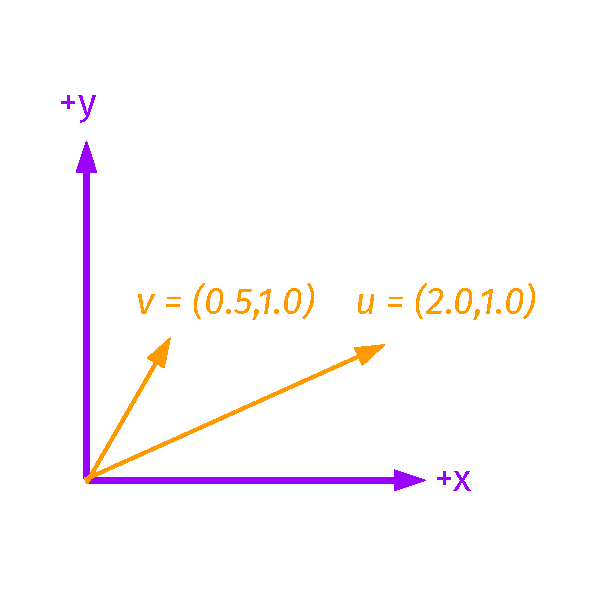
\includegraphics[width=0.45\textwidth,trim=1cm 1cm 1cm 1cm,clip=true]{figures/Vectors1.pdf}}
\subfloat[\label{fig:twovectors_b}]{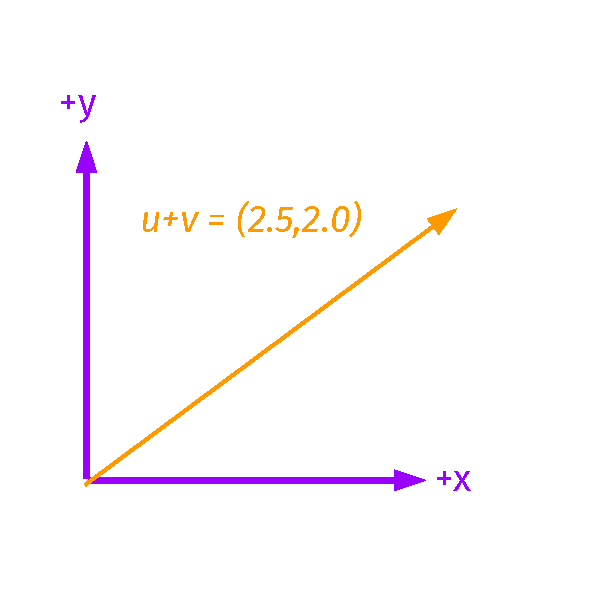
\includegraphics[width=0.45\textwidth,trim=1cm 1cm 1cm 1cm,clip=true]{figures/Vectors2.pdf}}
\caption{\label{fig:twovectors} (a) Two vectors in a two-dimensional Cartesian coordinate system: $\vec{u} = 0.5\hat{i}+1.0\hat{j}$ and $\vec{v} = 2.0\hat{i}+1.0\hat{j}$.  (b) What is $\vec{u}+\vec{v}$?  Adding components: $\vec{u}+\vec{v} = 2.5\hat{i}+2.0\hat{j}$.}
\end{figure}
\end{frame}

\begin{frame}{Coordinates and Vectors (Chapters 3.1 - 3.3)}
\begin{figure}
\centering
\subfloat[\label{fig:twovectors_c}]{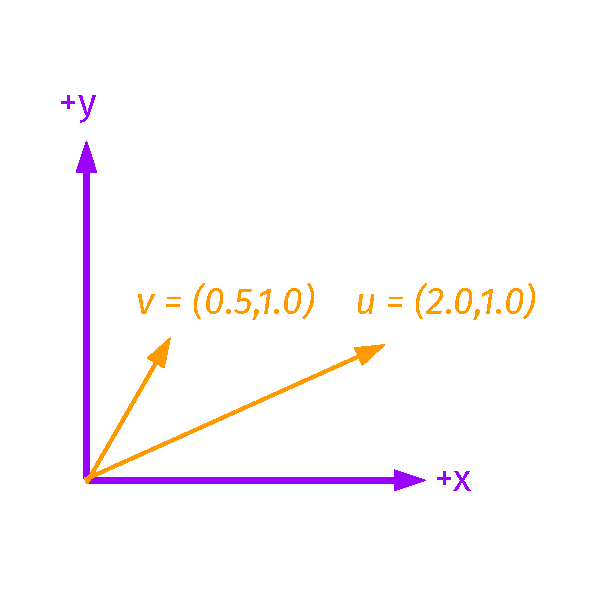
\includegraphics[width=0.45\textwidth,trim=1cm 1cm 1cm 1cm,clip=true]{figures/Vectors1.pdf}}
\subfloat[\label{fig:twovectors_d}]{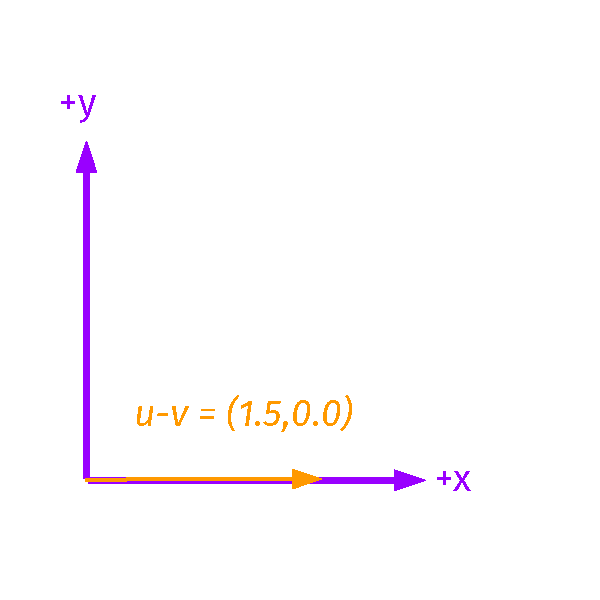
\includegraphics[width=0.45\textwidth,trim=1cm 1cm 1cm 1cm,clip=true]{figures/Vectors3.pdf}}
\caption{\label{fig:twovectors2} (a) Two vectors in a two-dimensional Cartesian coordinate system: $\vec{u} = 0.5\hat{i}+1.0\hat{j}$ and $\vec{v} = 2.0\hat{i}+1.0\hat{j}$.  (b) What is $\vec{u}-\vec{v}$?  Subtracting components: $\vec{u}-\vec{v} = 1.5\hat{i}+0.0\hat{j}$.}
\end{figure}
\end{frame}

\begin{frame}{Coordinates and Vectors (Chapters 3.1 - 3.3)}
\begin{figure}
\centering
\subfloat[\label{fig:twovectors_e}]{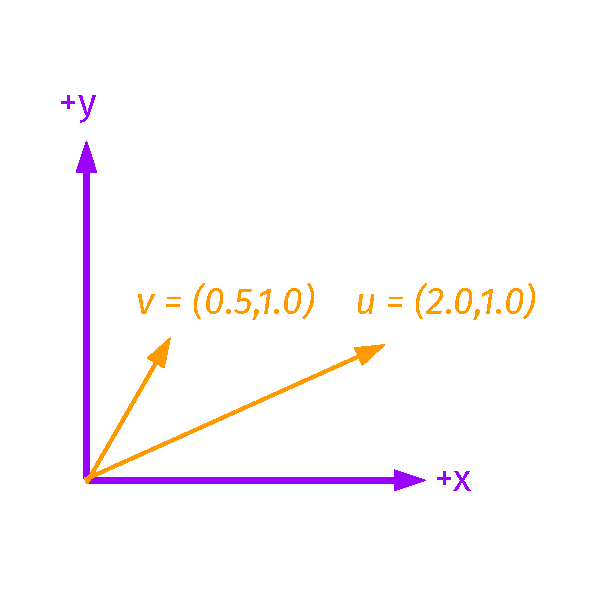
\includegraphics[width=0.45\textwidth,trim=1cm 1cm 1cm 1cm,clip=true]{figures/Vectors1.pdf}}
\subfloat[\label{fig:twovectors_f}]{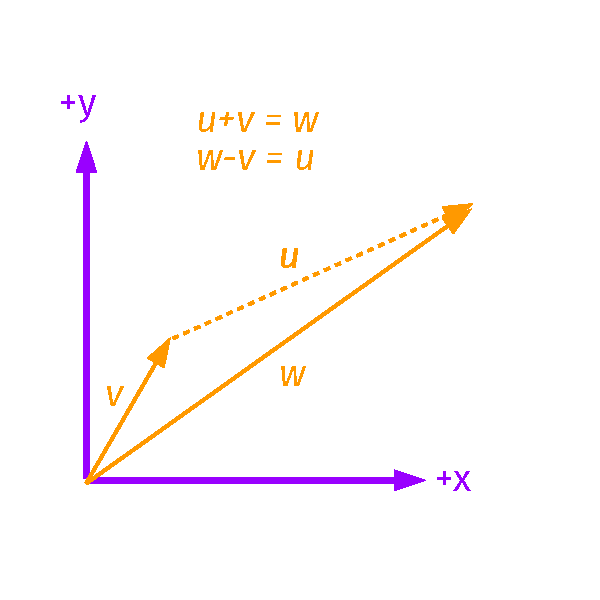
\includegraphics[width=0.45\textwidth,trim=1cm 1cm 1cm 1cm,clip=true]{figures/Vectors4.pdf}}
\caption{\label{fig:twovectors3} (a) Two vectors in a two-dimensional Cartesian coordinate system: $\vec{u} = 0.5\hat{i}+1.0\hat{j}$ and $\vec{v} = 2.0\hat{i}+1.0\hat{j}$.  (b) To compute $\vec{w}-\vec{v}$, arrange the vectors to get a sense of the result, $\vec{u}$.}
\end{figure}
\end{frame}

\begin{frame}{Coordinates and Vectors (Chapters 3.1 - 3.3)}
\small
\begin{minipage}[b]{0.45\linewidth}
Suppose $\vec{x}_i = -3\hat{i} + 2\hat{j}$ km, and $\vec{x}_f = -3\hat{i} - 2\hat{j}$ km.  What is the \textit{displacement}?
\vspace{0.2cm}
\begin{itemize}
\item A: $4\hat{i}$ km
\item B: $-4\hat{i}$ km
\item C: $4\hat{j}$ km
\item D: $-4\hat{j}$ km
\end{itemize}
\end{minipage}
\hspace{0.5cm}
\begin{minipage}[b]{0.45\linewidth}
Suppose $\vec{x}_i = 3\hat{i} - 2\hat{j}$ km, and $\vec{x}_f = 3\hat{i} - 2\hat{j}$ km.  What is the \textit{displacement}?
\vspace{0.2cm}
\begin{itemize}
\item A: 0 km
\item B: $0\hat{i} + 0\hat{j}$ km
\item C: $1\hat{i}$ km
\item D: $1\hat{j}$ km
\end{itemize}
\end{minipage}
\end{frame}

\begin{frame}{Coordinates and Vectors (Chapters 3.1 - 3.3)}
We define the \textit{position} of an object as a vector locating it in a given coordinate system.  The scalar \textit{distance} is the norm of the position vector, that is, the distance to to the origin. \\
\vspace{0.5cm}
Now we can introduce the concept of \alert{displacement}: a vector describing a movement of an object.
\end{frame}

\begin{frame}{Coordinates and Vectors (Chapters 3.1 - 3.3)}
\begin{figure}
\centering
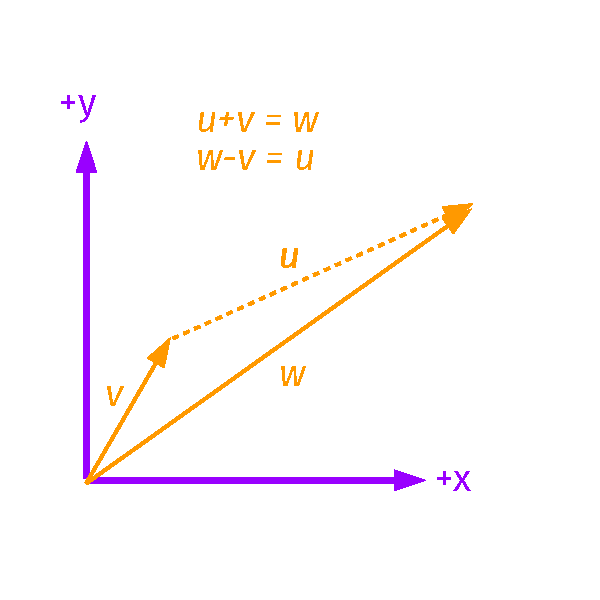
\includegraphics[width=0.52\textwidth]{figures/Vectors4.pdf}
\caption{\label{fig:displacement} Suppose an object moves from position $\vec{v}$ to $\vec{w}$.  In this case, the \alert{displacement} is $\vec{u}$. \textbf{Thus, the final position is the initial position, plus the displacement.}}
\end{figure}
\end{frame}

\begin{frame}{Coordinates and Vectors (Chapters 3.1 - 3.3)}
It follows that the \textit{displacement} is zero if the initial and final positions are the same, but the \textit{distance travelled} is not.\\
\vspace{0.2cm}
\small
Suppose a jet fighter travelling at 800 km per hour banks such that it flies in a circle of radius 0.5 km.  How long does it take to complete the circle?  What is the distance traveled, and what is the displacement?
\begin{itemize}
\item A: $2\pi$ km, 28 seconds, $2\pi$ km
\item B: $\pi$ km, 14 seconds, $\pi$ km
\item C: $\pi$ km, 28 seconds, $\pi$ km
\item D: $\pi$ km, 14 seconds, $0$ km
\end{itemize}
\end{frame}

\begin{frame}{Coordinates and Vectors (Chapters 3.1 - 3.3)}
\alert{Average velocity} is the ratio of the \alert{displacement} to the elapsed time.\\
\begin{equation}
\boxed{\vec{v}_{\rm avg} = \frac{\Delta \vec{x}}{\Delta t}}
\end{equation}
The \textit{average speed} is the norm of the average velocity:
\begin{equation}
\boxed{v_{\rm avg} = \frac{|\Delta \vec{x}|}{\Delta t}}
\end{equation}
If the motion is in one dimension, then the average speed is
\begin{equation}
v_{\rm avg} = \frac{x_{\rm f} - x_{\rm i}}{t_{\rm f} - t_{\rm i}}
\end{equation}
\end{frame}

\begin{frame}{Coordinates and Vectors (Chapters 3.1 - 3.3)}
\small
\begin{minipage}[b]{0.45\linewidth}
$\vec{p} = 4\hat{i}+2\hat{j}$.  $\vec{q} = -4\hat{i}+2\hat{j}$.  \\
Compute $\vec{p} \cdot \vec{q}$.
\vspace{0.2cm}
\begin{itemize}
\item A: 12
\item B: -12
\item C: 4
\item D: 8
\end{itemize}
\end{minipage}
\hspace{0.5cm}
\begin{minipage}[b]{0.45\linewidth}
$\vec{p} = -1\hat{i}+6\hat{j}$.  $\vec{q} = 3\hat{i}+0.5\hat{j}$.  \\
Compute $\vec{p} \cdot \vec{q}$.
\vspace{0.2cm}
\begin{itemize}
\item A: -1
\item B: 1
\item C: 0
\item D: 3
\end{itemize}
\end{minipage}
\end{frame}

\begin{frame}{Coordinates and Vectors (Chapters 3.1 - 3.3)}
Why was the last answer zero?  Look at it graphically:
\begin{figure}
\centering
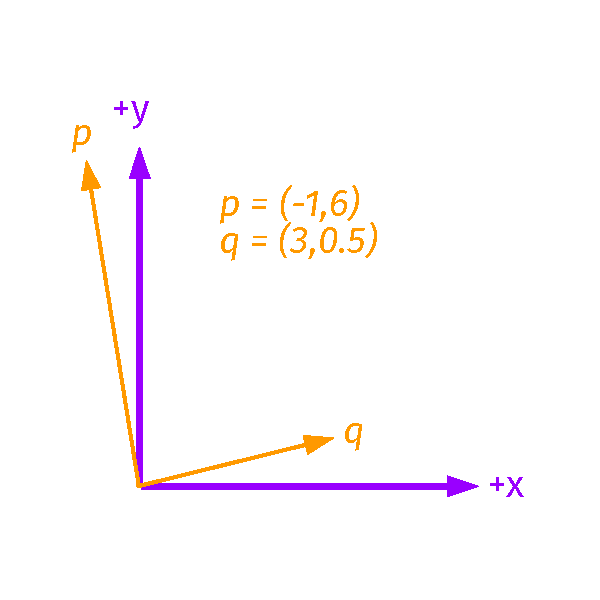
\includegraphics[width=0.5\textwidth,trim=1cm 1cm 1cm 1cm,clip=true]{figures/Vectors5.pdf}
\caption{\label{fig:twovectors4} Two vectors $\vec{p}$ and $\vec{q}$ are \textit{orthogonal} if $\vec{p} \cdot \vec{q} = 0$.}
\end{figure}
\end{frame}

\begin{frame}{Coordinates and Vectors (Chapters 3.1 - 3.3)}
The \textit{length} or \textit{norm} of a vector $\vec{v} = a\hat{i}+b\hat{j}$ is $|\vec{v}| = \sqrt{a^2+b^2}$.\\
\begin{figure}
\centering
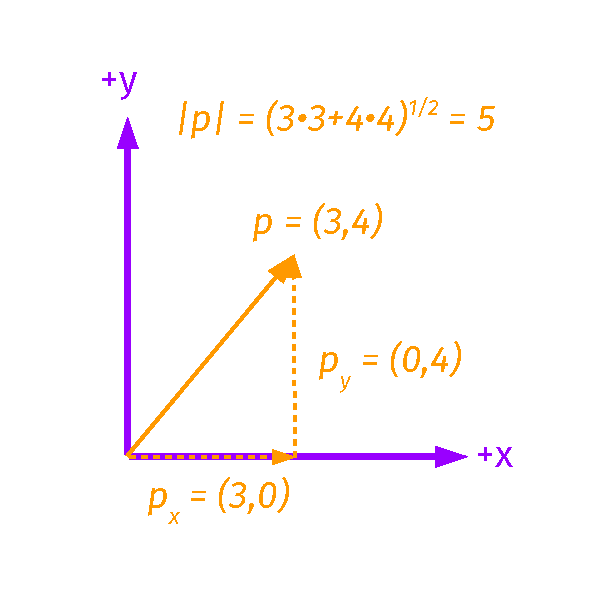
\includegraphics[width=0.5\textwidth,trim=1cm 1cm 1cm 1cm,clip=true]{figures/Vectors7.pdf}
\caption{\label{fig:twovectors6} Computing the norm of a vector $\vec{p}$.}
\end{figure}
\end{frame}

\begin{frame}{Coordinates and Vectors (Chapters 3.1 - 3.3)}
Notice that $\sqrt{\vec{p}\cdot\vec{p}} = |\vec{p}|$.\\
Let $\theta_p$ be the angle between $\vec{p}$ and the x-axis.  \\
$p_{x} = \vec{p} \cdot \hat{i} = |\vec{p}| \cos(\theta_{p})$. \\
$p_{y} = \vec{p} \cdot \hat{j} = |\vec{p}| \sin(\theta_{p})$.\\
\vspace{0.5cm}
\textit{Theorem:} The dot product of two vectors $\vec{p}$ and $\vec{q}$ is $|u||v|\cos(\theta)$, if $\theta$ is the angle between them.\\
\vspace{0.5cm}
\textit{Proof}: $\vec{p}\cdot\vec{q} = p_{x}q_{x} + p_{y}q_{y} = |p||q|\cos\theta_p\cos\theta_q+|p||q|\sin\theta_q\sin\theta_q$ \\
$=|p||q|(\cos\theta_p\cos\theta_q+\sin\theta_p\sin\theta_q) = |p||q|\cos(\theta_p-\theta_q)$ \\
$=|p||q|\cos\theta$. \\
\vspace{0.1cm}
$\boxed{\vec{p}\cdot\vec{q}=|p||q|\cos\theta}$
\end{frame}

\begin{frame}{Coordinates and Vectors (Chapters 3.1 - 3.3)}
\small
\begin{minipage}[b]{0.45\linewidth}
An object moves at 2 m/s at $\theta = 60^{\circ}$ with respect to the x-axis.  What is the velocity of the object?
\vspace{0.2cm}
\begin{itemize}
\item A: $(1\hat{i}$ + $1\hat{j})$  m/s
\item B: $(\sqrt{3}\hat{i}$ + $1\hat{j})$  m/s
\item C: $(\sqrt{3}\hat{i}$ + $\sqrt{3}\hat{j})$  m/s
\item D: $(1\hat{i}$ + $\sqrt{3}\hat{j})$  m/s
\end{itemize}
\end{minipage}
\hspace{0.5cm}
\begin{minipage}[b]{0.45\linewidth}
An object moves at 2 m/s at $\theta = 120^{\circ}$ with respect to the x-axis.  What is the velocity of the object?
\vspace{0.2cm}
\begin{itemize}
\item A: $(-1\hat{i} + \sqrt{3}\hat{j})$ m/s
\item B: $(1\hat{i} - \sqrt{3}\hat{j})$ m/s
\item C: $(-1\hat{i} + \sqrt{3}\hat{j})$ m/s
\item D: $(-1\hat{i} - \sqrt{3}\hat{j})$ m/s
\end{itemize}
\end{minipage}
\end{frame}

\begin{frame}{Coordinates and Vectors (Chapters 3.1 - 3.3)}
Is it possible to multiply vectors and scalars?  Of course: $a_1\vec{p} = a_1p_x\hat{i}+a_1p_y\hat{j}$.\\
\vspace{0.2cm}
Also, multiplication properties still hold.  For example: $(a_1+a_2)\vec{p} = a_1\vec{p}+a_2\vec{p}$. \\
\vspace{0.2cm}
\small
A spacecraft moves at 400 m/s, at an angle of 30 degrees with respect to the x-axis.  If it fires two thrusters that boost the x-component and y-component of the velocity by 25\% and 50\%, respectively, what is the final velocity?
\begin{itemize}
\item A: $(433\hat{i}+300\hat{j})$ m/s
\item B: $(300\hat{i}+433\hat{j})$ m/s
\item C: 400 m/s
\item D: $(400\hat{i}+433\hat{j})$ m/s
\end{itemize}
\end{frame}

\begin{frame}{Coordinates and Vectors (Chapters 3.1 - 3.3)}
\begin{figure}
\centering
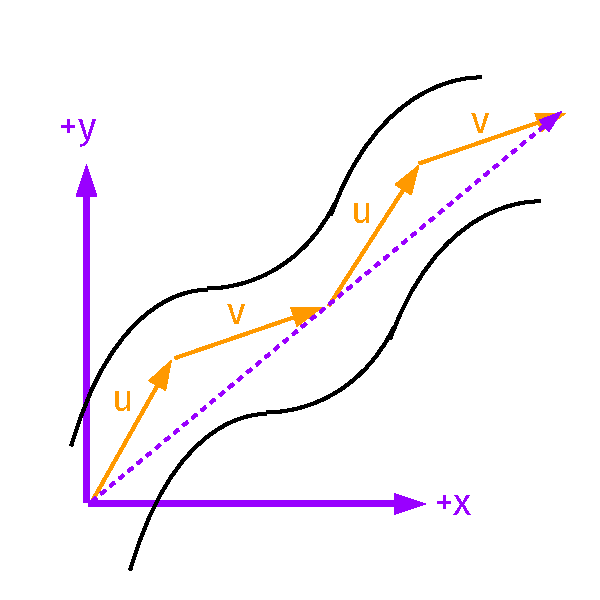
\includegraphics[width=0.52\textwidth]{figures/AveVelocity.pdf}
\caption{\label{fig:avevel} A Formula-1 driver keeps his car on the track by following a path approximated by the position vectors $u$, $v$, $u$, and $v$.  The dashed arrow represents the total displacement.}
\end{figure}
\end{frame}

\begin{frame}{Coordinates and Vectors - Average Velocity (Chapter 2.3)}
If $\vec{u} = (20\hat{i}+30\hat{j})$ m, and $\vec{v} = (30\hat{i}+20\hat{j})$ m, what is the total displacement?  If the elapsed time is 10 seconds, what is the magnitude of the average velocity? \\
\vspace{0.2cm}
\begin{itemize}
\item A: $(50\hat{i} + 50\hat{j})$ m, 14 m/s
\item B: $(80\hat{i} + 100\hat{j})$ m, 10 m/s
\item C: $(100\hat{i} + 100\hat{j})$ m, 14 m/s
\item D: $(50\hat{i} + 150\hat{j})$ m, 10 m/s
\end{itemize}
\end{frame}

\begin{frame}{Coordinates and Vectors (Chapters 3.1 - 3.3)}
PhET simulation about vector addition: \\
\url{https://phet.colorado.edu/en/simulation/vector-addition}
\end{frame}

\section{Kinematics and Newton's Laws}

\begin{frame}{Kinematics and Newton's Laws}
\small
\textit{Kinematics} - A \alert{description} of the motion of particles and systems \\
\textit{Dynamics} - An \alert{explanation} of the motion of particles and systems \\
\vspace{0.25cm}
What causes an object to move?  \textbf{Forces}.  Forces exist as a result of the \alert{\textbf{interactions}} of objects or systems.\\
\vspace{0.25cm}
\rule{10cm}{0.4pt} \\
\vspace{0.25cm}
\textit{Evolution} - A \alert{description} of the change of biological species \\
\textit{Natural Selection} - An \alert{explanation} of change in biological species \\
\vspace{0.25cm}
What causes species to evolve?  \textbf{Natural selection}.  Natural selection exists because of \alert{election pressures}, \alert{numerous offspring}, and \alert{variation} among offspring.
\end{frame}

\begin{frame}{Kinematics and Newton's Laws}
\textbf{Newton's First Law}: A man slides a palette crate across a concrete floor of his shop.  He exerts a force of 60.0 N, and the box has a constant velocity of 0.5 m/s.  What force cancels his pushing force, and what is the value in Newtons?
\begin{itemize}
\item A: wind, 60.0 N
\item B: friction: 60.0 N
\item C: friction: -60.0 N
\item D: weight: -60.0 N
\end{itemize}
\end{frame}

\begin{frame}{Kinematics and Newton's Laws}
\textbf{Newton's Second Law}: The crate has a mass of 50 kg, and encounters an area where there is no longer friction.  If the pushing force is still 60 N, what is the acceleration?
\begin{itemize}
\item A: 1.0 m/s$^2$
\item B: 0.8 m/s
\item C: 1.2 m/s
\item D: 1.2 m/$^2$
\end{itemize}
\end{frame}

\begin{frame}{Kinematics and Newton's Laws}
\textbf{Kinematics}: If the acceleration is 1.2 m/s$^2$, and the crate begins with a velocity of 1 m/s, what is the velocity after 5 seconds?
\begin{itemize}
\item A: 4 m/s
\item B: 5 m/s
\item C: 6 m/s
\item D: 7 m/s
\end{itemize}
\end{frame}

\begin{frame}{Kinematics and Newton's Laws}
\textbf{Newton's Second Law}: Suppose there is no pushing force, but the crate moves at 5 m/s through an area with a frictional force that has a magnitude of 5 N.  If the crate still weighs 50 kg, what is the acceleration?
\begin{itemize}
\item A: 0.2 m/s$^2$
\item B: -0.1 m/s$^2$
\item C: 1 m/s$^2$
\item D: -2 m/s$^2$
\end{itemize}
\end{frame}

\begin{frame}{Kinematics and Newton's Laws}
\textbf{Newton's Third Law}: If a person hangs from a horizontal rope (with the ends tied to two walls), and the person has a weight $\vec{w} = -600 N$, what is the total upward component of the tension in the rope?
\begin{itemize}
\item A: -600 N
\item B: 60 N
\item C: 600 N
\item D: -60 N
\end{itemize}
\end{frame}

\begin{frame}{Kinematics and Newton's Laws}
\textbf{Newton's Third Law}: If a heavy truck and a light car collide, which exerts the larger force on the other?
\begin{itemize}
\item A: The heavy truck exerts a larger force on the car.
\item B: The light car exerts a larger force on the heavy truck.
\item C: They exert the same force on each other.
\item D: Cannot determine.
\end{itemize}
\end{frame}

\section{Work-Energy Theorem and Conservation of Energy}

\begin{frame}{Kinetic Energy and the Work-Energy Theorem}
\textbf{Group board exercise}: A firework of mass 1 kg is launched straight upwards.  The gunpowder releases 500 J of energy.  What is the velocity of the shell as it leaves the launcher?  How high does it fly straight upwards? \\ \vspace{0.5cm}
Three useful concepts: 1) Work equation 2) Work-energy theorem 3) gravitational potential energy.
\end{frame}

\begin{frame}{Kinetic Energy and the Work-Energy Theorem}
\textbf{Work-energy theorem}: How high in the air would a 0.1 kg rock go if it was launched straight upward by a spring with $k=1000$ N/m, if the spring was compressed $0.1$ m?
\begin{itemize}
\item A: 0.5 m
\item B: 5 m
\item C: 50 m
\item D: 500 m
\end{itemize}
Note: the potential energy of a spring with spring constant $k$ and displacement $x$ is $U = \frac{1}{2}k x^2$.
\end{frame}

\begin{frame}{Kinetic Energy and the Work-Energy Theorem}
\textbf{Work-energy theorem}: How high would it go if the spring was compressed $0.2$ m?
\begin{itemize}
\item A: 100 m
\item B: 200 m
\item C: 500 m
\item D: 50 m
\end{itemize}
Note: think of this exercise as a scaling problem.
\end{frame}

\section{Momentum}

\begin{frame}{Momentum}
A ball with mass 0.1 kg moves at 1 m/s.  It strikes a stationary ball with twice the mass and stops.  The heavier ball moves with a velocity of
\begin{itemize}
\item A: 0.1 m/s
\item B: 1 m/s
\item C: 5 m/s
\item D: 0.5 m/s
\end{itemize}
\end{frame}

\begin{frame}{Momentum}
A ball with mass 0.1 kg moves at 1 m/s.  It strikes a stationary ball with the same mass and they stick together.  What is the final velocity of the object?
\begin{itemize}
\item A: 0.1 m/s
\item B: 1 m/s
\item C: 5 m/s
\item D: 0.5 m/s
\end{itemize}
\end{frame}

\begin{frame}{Momentum}
If the mass of an object that is rotating around an origin with angular velocity $\omega$ decreases by a factor of 2, the new angular velocity will be:
\begin{itemize}
\item A: $-\omega$
\item B: $-3\omega$
\item C: $2\omega$
\item D: $\omega$
\end{itemize}
\end{frame}

\section{Electrostatics I}

\section{Electrostatics II}

\section{Conclusion}

\begin{frame}{Unit 0 Summary}
\textbf{Reading: Chapters 3.1 - 3.3, 18.1 - 18.5, 19.1 - 19.3}
\begin{enumerate}
\item Estimation/Approximation
\item Coordinates and Vectors
\item Review of concepts from Newtonian mechanics
\begin{itemize}
\item Kinematics and Newton's Laws
\item Work-energy theorem, energy conservation
\item Momentum, conservation of momentum
\end{itemize}
\item Electrostatics I: charges and fields
\item Electrostatics II: potential, and potential energy
\end{enumerate}
\end{frame}

\end{document}
